\documentclass{article}
\usepackage{graphicx}
\usepackage{float}

\begin{document}
\pagenumbering{gobble}
    \begin{titlepage}
    \begin{center}
        \textbf{VILNIUS UNIVERSITY}\\
        \textbf{FACULTY OF MATHEMATICS AND INFORMATICS}\\
        \vspace*{1cm}
        \textbf{Team Agreement}\\
    \end{center}
    \vspace*{5cm}
    \begin{flushright}
        \textbf{Team members:}
        Rytis Tauras, Emil Duko, Žygimantas Vidmantas,\\Matas Čeplinskas
    \end{flushright}
    \vfill
    \begin{center}
        2025-09-10
    \end{center}
\end{titlepage}
    \newpage
    \pagenumbering{arabic}
    
    \section{Introduction}
    This document depicts the technical description of a point of sales (POS) software system for small and medium businesses in catering (bars/cafe/restaurants) and beauty (barbers/hairdressers/SPA) sectors.\\[0.2cm] Key features of the system include:
    \begin{itemize}
        \item creating an account for your business by picking the sector it represents
        \item adding employees and their log in information 
        \item creating and modifying items that would represent your business' catering or services menu
        \item adding tax information, discounts and gift cards
        \item payment system that supports check splitting, tip adding and cash, credit/debit cards or gifts cards payments
        \item booking system for tables? or service appointments
        \item order or service appointment management system for modifying or canceling them
        \item inventory management system
        \item sms notifications system for booked appointments
    \end{itemize}

    \section{Business flows}
    \subsection{Business owner workflow}
    \subsubsection{Business account creation}
    This section describes how a business owner modifies their business account information in the PoS system.\\
     If owner wants to modify some of the business information fields (address, contact info - phone/email, name), he can do so after logging into his account, selecting the account tab and pressing the edit business information button. Then the server updates the modified fields.
    \begin{figure}[H]
        \centering
        \includegraphics[width=0.9\linewidth]{PSP/lab-1/mockups/account.png}
        \caption{business owner account tab}
        \label{}
    \end{figure}

     
    \subsubsection{User management}
    This section describes how one can manage access to the PoS system. The ability to edit employees/users of their business is available only to logged-in and authorized business owner or super admin (IT support) that can edit anyone.\\
    The process starts by the server accessing employee data and showing it in the interface. Firstly, the manager can add a new employee by clicking the add employee button in the employees tab and filling in necessary fields of information for its creation and then the server creates the record with an "active" status. Otherwise, if he is trying to edit or delete an employee, he has to pick which employee is gonna get processed and click either of suggested buttons, so then the server updates employees record with new fields or "inactive" status.
    \begin{figure}[H]
        \centering
        \includegraphics[width=0.9\linewidth]{PSP/lab-1/mockups/employees.png}
        \caption{employee tab}
        \label{}
    \end{figure}
    
    \subsection{Manager workflow}
    \subsubsection{Menu management} %add mockup
    This section describes how one can manage businesses' product/item menu. The ability to edit, delete or create new items in the menu is available only to logged-in and authorized business owner or product manager.\\
    The process starts by the server accessing menu data and displaying it in the interface. Firstly, the manager is able to pick from the options of creating a new item or either deleting or editing an existing one. Secondly, if he is creating an item the manager has to fill in necessary fields of information for its creation and then the server creates it and adds to the menu. Otherwise, if he is trying to edit or delete one, he has to pick which item is gonna get processed and then the server updates the items fields or removes the item from the menu.
    % mockup
    
    \subsubsection{Refund management}
    This section describes how one can refund an order in the PoS system. This ability is available only to logged-in and authorized business owner or any kind of manager and only closed orders can be refunded.\\ 
    The process starts by the manager selecting to open orders tab and then the server accesses and returns closed orders list and displays it in the interface. Then, he has to select a specific order from the list and its information is shown while also the refund option appears. After clicking the refund button, manager has to pick if it is a full or a partial refund. If it is a partial refund manager has to input the amount, otherwise it just processes the full order payment amount and then the server updates order information with a "refunded" status and manager who initiated the refund id .%add card options 
    \begin{figure}[H]
        \centering
        \includegraphics[width=0.9\linewidth]{PSP/lab-1/mockups/orders.png}
        \caption{orders tab}
        \label{}
    \end{figure}
    
    \begin{figure}[H]
        \centering
        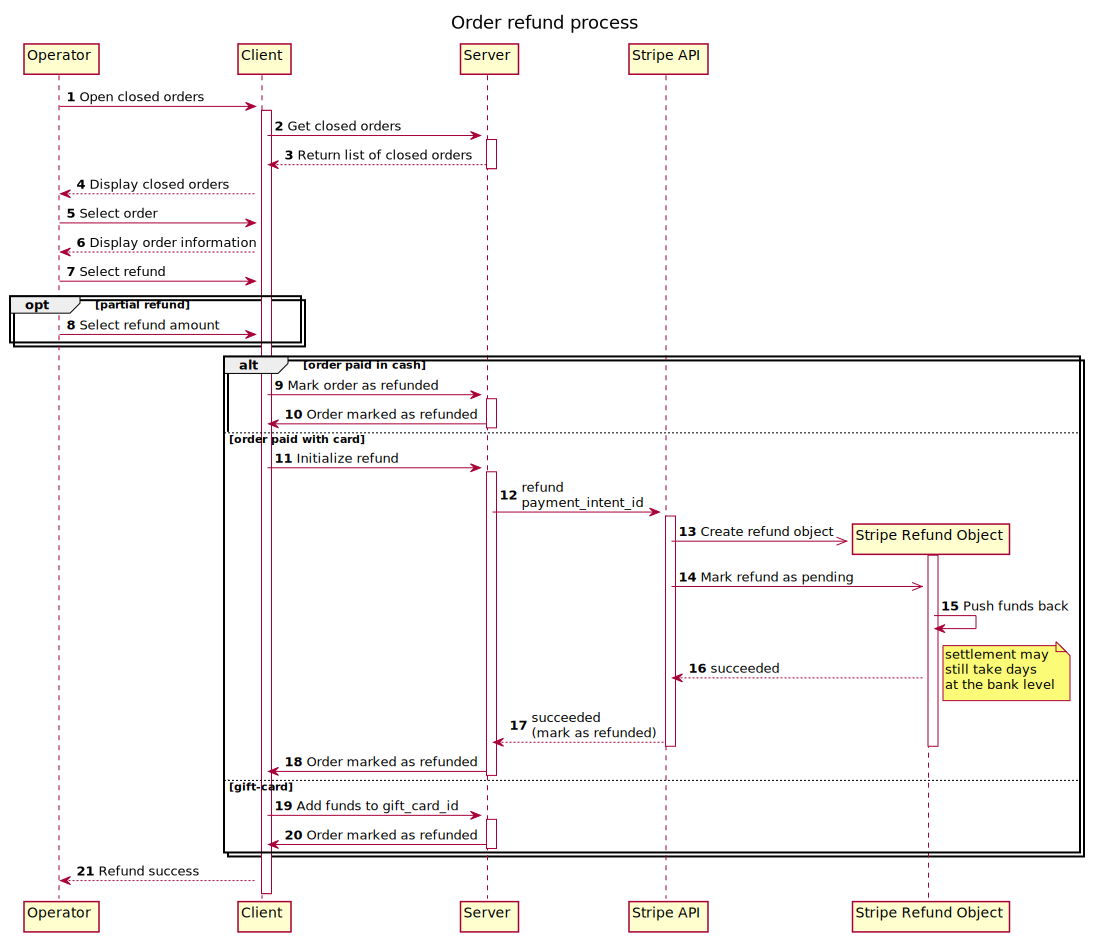
\includegraphics[width=0.9\linewidth]{PSP/lab-1/diagrams/sequence/refund.png}
        \caption{}
        \label{}
    \end{figure}

    \subsubsection{Inventory management} % add mockup
    This section describes how one can manage businesses' inventory. The ability to edit the inventory amounts is available only to logged-in and authorized business owner or inventory manager.\\
    Firstly, user has to open the inventory tab where he can see items and their number in stock that goes down automatically after an order is processed. He can also edit the numbers by clicking on any item and typing a number in, in case of a restock.

    \subsection{Employee workflow}
    \subsubsection{Order system}
    This section describes how an employee creates and modifies orders in the PoS system. This ability is available only to logged-in users.\\
    The process starts by the employee wanting to create a new order and then new order entity with unique id is created that appears empty in the interface and employee has to add items and their amount from the item menu into it. With each add the item and its quantity is displayed on the screen in the order information. Then employee also has the option to remove any item from the displayed order, while it is not confirmed. After making sure he got everything, employee confirms the order by pressing the proceed button and it is sent to the server, then it is considered "pending" and payment options become active. However, before the order is confirmed there is an option to cancel it all together.
     \begin{figure}[H]
        \centering
        \includegraphics[width=0.9\linewidth]{PSP/lab-1/mockups/hometab.png}
        \caption{home tab}
        \label{}
    \end{figure}
    
    \begin{figure}[H]
        \centering
        \includegraphics[width=0.9\linewidth]{PSP/lab-1/diagrams/sequence/order.png}
        \caption{}
        \label{}
    \end{figure}

    \begin{figure}[H]
        \centering
        \includegraphics[width=0.9\linewidth]{PSP/lab-1/diagrams/sequence/service-order.png}
        \caption{}
        \label{}
    \end{figure}
    
    \subsubsection{Payment system} %add mockup
    This section describes how payments and tips are handled in the PoS system. This functionality is available only to logged-in users.\\
    After taking the order and clicking the proceed button the payment window appears, where the user is able to select between card or cash payment, or if a gift card code was entered previously, the amount in that card would be deducted from the bill. Also, before the said payment, there is an option to split the bill into different parts and pay those parts by different payment methods mentioned previously.
    \begin{figure}[H]
        \centering
        \includegraphics[width=0.7\linewidth]{PSP/lab-1/diagrams/sequence/payment.png}
        \caption{}
        \label{}
    \end{figure}
    
    \subsubsection{Appointment/booking system}
    This section describes how service appointments are handled in the PoS system. This functionality is available only to logged-in users.\\
    
    \section{High level architecture}
        \begin{figure}[H]
        \centering
        \includegraphics[width=0.9\linewidth]{PSP/lab-1/diagrams/architecture/package-diagram.png}
        \caption{High level component relation model}
        \label{}
        \end{figure}
    \section{Data model}
    \begin{figure}[H]
        \centering
        \includegraphics[width=1.0\linewidth]{PSP/lab-1/diagrams/data-model/data-model.png}
        \caption{class relations model}
        \label{}
        \end{figure}
    \section{API Contracts for the backend endpoints}

    List: ( before putting properly in .yaml)\\
    GET /organisations\\
    GET /organisations/{organisationId} \\
    POST /organisations - Add organisation\\
    PATCH /organisations/{organisationId}\\
    GET /organisations/{organisationId}/menu-items\\
    GET /menu-items/{itemId}\\
    
    
\end{document}